%%%%%%%%%%%%%%%%%%%%%%%%%%%%%%%%%%%%%%%%%%%%%%%%%%%%%%%%%
\chapter{Time dependent circuits}
So far, we have not considered how electrical networks (circuits) depend on time. Once the circuit is plugged in, we have just assumed the network instantly takes on  the appropriate currents and voltages. This is appropriate for circuits containing ideal voltage sources, current sources and resistors, but real circuits contain other components whose behavior depend on time.\\

\begin{alevel}
What do AC and DC stand for?
\end{alevel}

%%%%%%%%%%%%%%%%%%%%%%%%%%%%%%5555
\section{Capacitors, RC circuits}
This chapter introduces two components whose voltage-current relationship depends on time. Table~\ref{T:6RLC} shows how they behave:

\begin{table}[H]
\begin{center}
\renewcommand{\arraystretch}{1.5}
\begin{tabular}{|c|c|c|} \hline
component	& current		&	voltage	\\ \hline
resistor	&$I=\frac{\Delta V}{R}$	&$\Delta V=IR$	\\ \hline
capacitor	&$I=C\frac{d\Delta V}{dt}$	&$\Delta V=?$	\\ \hline
inductor	&I=?			&$\Delta V=L\frac{dI}{dt}$	\\ \hline
\end{tabular}
\caption{I-V relationships for R, L and C}
\label{T:6RLC}
\end{center}
\end{table}

The constants `C' and `L' represent capacitance and inductance.\par

Let's fill in the two remaining blanks. For the capacitor, we need to rearrange the current equationt to solve for $\Delta V$, but the rearrangement requires a little calculus:

\begin{align*}
I&=C\frac{dV_C}{dt}\\
Idt &= CdV &&\text{Multiply by dt}\\
\int{Idt} &= C \int dV_C\\
\frac{1}{C} \int Idt &= V_{Cf}-V_{Ci}\\
V_C&=\frac{1}{C} \int{Idt} &&\text{if $V_{Ci}=0$}
\end{align*} 

See footnote.\footnote{Both $V_{Cf}$ and $V_{Ci}$ themselves represent the change in voltage from one side of the capacitor to the other. I could have written them as $\Delta V_{Cf}$ and $\Delta V_{Ci}$, but that might be confusing because you might think of $\Delta V_C$ as the change in voltage over time, which is $V_{Cf}-V_{Ci}$. Alas, I suppose it's a little confusing either way.}

\begin{alevel}
What are the S.I. units of inductance.
\end{alevel}

\begin{clevel}
Rearrange the inductor equation to solve for the current through the inductor as a function of time.
\end{clevel}

\begin{blevel}
The current through a 5H inductor changes with time according to $I=(3t^2+5)$ Amps. Determine the voltage across this inductor as a function of time. 
\end{blevel}

\begin{clevel}
The current onto a 5F capacitor changes with time according to $I=(3t^2+5)$ Amps. The initial voltage across the capacitor is 2V. Determine the voltage across this capacitor as a function of time. 
\end{clevel}

%%%%%%%%%%%%%%%%%%%%%%%%%%%%%%%%%%%%%%%%%%%%%%%%%%%%%%%%%%%%%%%%%%%%%%%%%%%%%
\subsection{The Capacitor: An Electric Spring}
A simple capacitor consists of a pair of two parallel plates separated by a non-conducting material, like an air gap. Figure~\ref{F:6CAP0} shows a basic parallel plate capacitor. 
\\
\begin{figure}[H]
\begin{center}
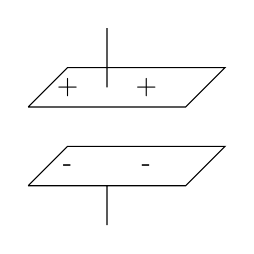
\begin{tikzpicture}
\draw (0,0)--(2,0)--(2.5,.5)--(.5,.5)--(0,0) (1,0)--(1,-.5);
\draw (0,1)--(2,1)--(2.5,1.5)--(.5,1.5)--(0,1) (1,1.25)--(1,2);
\draw node at (.5,1.25) {+};
\draw node at (1.5,1.25) {+};
\draw node at (.5,.25) {-};
\draw node at (1.5,.25) {-};
\end{tikzpicture}
\caption{A parallel plate capacitor. The charges represent continuous films of charge.}
\label{F:6CAP0}
\end{center}
\end{figure}

\textbf{Question:} Do charges like to accumulate on the plates of a capacitor?\par
\textbf{Answer:} No. Imagine smooshing a film of positive charge on one side and an equal amount of negative charge on the other. While it is true that the positive charges attract the negative charge on the other side of the plate, the continuous film of positive charges are very close to each other and repel each other more than attract to the negative charges.\par
\textbf{Follow-up Question:} ...but charge is quantized. Therefore the electrons on the negative side can spread out and their spacing might exceed the spacing of the plates. Like if we put 4 electrons on one plate and four protons on the other, they'd all run to the corners and attract the electrons. Wouldn't that make them want to be there? \par
\textbf{Answer:} Sure, but the gap would need to be really small for that effect to need consideration. If you spread 1 C of electrons across a 1 square meter surface, the electrons would be about a half a nanometer apart from each other.\footnote{And even then if it were energetically favorable for a few charges to be attracted to the plates, these charges would just always be there, and wouldn't effect our analysis.}\par
\textbf{Key Point:} You need to push charges onto a capacitor, like pushing air into a balloon. If you let them, the charges will prefer to leave the capacitor.\par

A capacitor acts like a spring. For a spring, the force needed to compress it further depends on how much the spring is already compressed, modeled mathematically as:\par

\begin{align}
\|F_{spring}\| = kx&& \text{or}&& F_{spring} \propto x
\end{align}

\begin{alevel}
A metal spring has a spring constant of 15 N/m and is already squished 1 cm. What force would be needed to squish it tiny bit more?
\end{alevel}

For a capacitor, the force needed to add extra charge depends on how much charge you want to add (put) and also on how much charge is already there \footnote{This can be motivated by Coulomb's Law, $F=\frac{kq_{put}q_{there}}{r^2}$, where $q_{put}$ and $q_{there}$ might represent the two charges (the amount your putting and the amount already there). Of course, $q_{there}$ probably wouldn't be well modeled as a point charge, but $F\propto q_{put}q_{there}$ should still hold. }.

Based on this, the following would be true:

\begin{enumerate}
\item The force needed to add more charge is proportional to the amount of charge already on the plates of the capacitor. \par 

\begin{align}
\|F\| \propto (q_{put})q_{there} \label{E:6CL0}
\end{align}

For a parallel plate capacitor, the force needed to pull a charge ($q_{put}$) from the negative plate towards the positive plate would be:
\begin{align*}
\vec{F}=q_{put}\vec{\mathcal{E}}=q_{put}\frac{\sigma_{plate}}{\epsilon}=\frac{q_{put}q_{there}}{A\epsilon}\\
\sigma_{plate} = \text{the charge already on the plates}
\end{align*}

\item The energy needed to add charge to the plates of a capacitor depends on the force \footnote{Other things matter, too, like the distance the charge needs to be moved and the arrangement of the plates (parallel, cylindrical, etc.).}.
\begin{align}
|PE\|  \propto (q_{put})q_{there} \notag
\end{align}
In the case of the parallel plate capacitor:
\begin{align*}
Work=\vec{F}\bullet \vec{d} = \frac{q_{put}q_{there}}{A\epsilon}t\\
t = \text{spacing between the plates}
\end{align*}

\item The energy required depends on how much charge we add. Therefore, instead of energy, it might make more sense to think in terms of energy per charge (voltage).
\begin{align}
\frac{PE}{q_{put}} \propto q_{there}&&\rightarrow&&V \propto q_{there} \notag \\
&&&&V= \frac{1}{C} q_{there} \label{E:6CL}
\end{align}
In the case of the parallel plate capacitor:
\begin{align*}
\frac{PE}{q_{put}} = \frac{q_{there}}{A\epsilon}t=q_{there}(\frac{t}{A\epsilon})\\
t = \text{spacing between the plates}
\end{align*}
\item The constant of proportionality is written as $\frac{1}{C}$, where C is the capacitance.
In the case of the parallel plate capacitor:
\begin{align*}
C = \frac{A\epsilon}{t}
\end{align*}
\end{enumerate}

\begin{alevel}
What are the S.I. units of capacitance. Look it up. 
\end{alevel}

\begin{blevel}
A 10F parallel plate capacitor has a voltage drop across it of 5 Volts. How much extra positive charge is on the top plate? How much extra negative charge is on the bottom plate?
\end{blevel}

\begin{blevel}
How much voltage is needed to push 5C of charge onto a 10F capacitor? How much voltage is needed to push 5C of charge onto a 2F capacitor? Is it easier to push charge onto a large capacitor or a smaller one?
\end{blevel}

\begin{clevel}
Suppose a 2C charge is located 3m away from a clump of 50C of charge. What force is needed to push the 2C charge just a tiny bit closer to the clump?
\end{clevel}

\begin{clevel}
A 3A current flows onto a 5F capacitor. At time zero there is no charge on the capacitor. What is the voltage across the capacitor after 2 seconds? After 4 seconds? After 6 seconds?
\end{clevel}

I want to repeat here that capacitors do not ``fill up" like water tanks. They are more like water balloons. It gets harder and harder to add charge to them as you crowd more charge onto them. If you put too much charge on them, they eventually break, like pulling too hard on a rubber band. The electric field between the plates increases with the amount of charge. When this field exceeds an amount called \emph{breakdown field}, the material between the capacitors starts to conduct, causing a surge in current which will overheat (or maybe melt) the capacitor.\footnote{Like a lightning bolt.}

\begin{blevel}
What is the breakdown electric field for air? What voltage drop across a 1 mm gap would cause such an electric field?
\end{blevel}

\subsection{The Capacitor I-V Relationship}
Let's manipulate Equation~\ref{E:6CL} so that we can see where the I-V relationship for a capacitor comes from:

\begin{align*}
V &= \frac{q}{C}&&\text{V means the voltage difference across C}\\
q &= CV\\
\frac{d}{dt}(q &= CV)\\
\frac{dq}{dt}&=C\frac{dV}{dt}\\
I &= C\frac{dV}{dt}
\end{align*}

Unlike a resistor, where the current depends on the voltage, the current through a capacitor depends on the change in voltage. If the voltage is constant, then the current would be zero.\par

\begin{alevel}
Is it possible for a car to have a zero acceleration, but a non-zero velocity? Is it possible for a car to have zero velocity, but a non-zero acceleration?
\end{alevel}

\begin{alevel}
Is it possible for a resistor to have no current through it, yet have non-zero voltage across it?
\end{alevel}

\begin{alevel}
Is it possible for a capacitor to have no current through it, yet have non-zero voltage across it?
\end{alevel}

\begin{clevel}
Suppose the voltage across a capacitor were $V = 5e^{3it}$, where i is $\sqrt{-1}$. What would be the units of the `5'? How about the units of the `3'?
\end{clevel}

\begin{clevel}
Suppose the voltage across a capacitor were $V = 5e^{3it}$. Determine the current onto the capacitor as a function of time.
\end{clevel}

%%%%%%%%%%%%%%%%%%%%%%%%%%%%%%%%%%%%%%%%%%%%%%%%%%
\subsection{Capacitors for storing energy}
Consider the total work needed to push some charges onto a capacitor. The first several charges are easy to push onto the capacitor because there is little repulsive force, but more work is needed as the capacitor fills up. Let's calculate the work done (using P=IV and $P=\frac{dE}{dt} = \frac{dW}{dt}$):

\begin{align*}
W &= \int{ P dt}\\
W &= \int{ IV dt}\\
W &= \int{ (C\frac{dV}{dt})Vdt}\\
W &=\int{ CVdV}\\
W &= \frac{1}{2}CV^2
\end{align*}

The work it takes to push charges onto a capacitor would also equal the maximum amount of energy that the capacitor could store. During the next several questions we will design a parallel plate capacitor that can store an amount of energy equivalent to one gallon of gas. The spacing between the plates will be set to 1 mm and the gap will be filled with air.

\begin{alevel}
How many Joules of energy would this be?
\end{alevel}

\begin{blevel}
If the spacing between the plates is 1mm, what is the max voltage that can be applied to the capacitor before the electric field exceeds the breakdown field of the air between the plates? Hint: See previous question about breakdown field.
\end{blevel}

\begin{blevel}
What size capacitance is needed?
\end{blevel}

\begin{blevel}
Look up a formula for the capacitance of a parallel plate formula and determine the area of the plates needed. Does this seem practical as an energy storage option for an electric car?
\end{blevel}

\begin{dlevel}
Derive the formula for the capacitance of a parallel plate capacitor. Number your steps.
\end{dlevel}

%%%%%%%%%%%%%%%%%%%%%%%%%%%%%%%%%%%%%%%%%%%%%%%%%%%%%%%%%%%%%%%%%%%%%%%%%%%%%%%
\section{Capacitor Circuits}
\subsection{A boring capacitor circuit}
Consider the circuit in Figure~\ref{F:6CA} consisting of a voltage source and a capacitor.\par

\begin{figure}[H]
\begin{center}
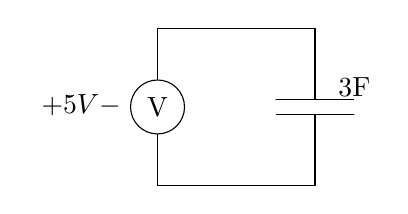
\begin{tikzpicture}
\draw (0,0)--(0,1) node[circle,draw=black, fill=white,radius=.1 mm, label=left:{}]{V}
--(0,2)--(2,2);
\draw (2,2)--(2,1.1)--(1.5,1.1)--(2.5,1.1) (1.5,.9)--(2.5,.9)--(2,.9)--(2,0)--(0,0);
\draw node at (2.5,1.25) {3F};
\draw node at (-1,1) {$\begin{matrix}+\\5V\\-\end{matrix}$};
\end{tikzpicture}
\caption{Voltage source connected to a capacitor}
\label{F:6CA}
\end{center}
\end{figure}

The instant we plug it in, the capacitor will immediately charge up to 5V (KVL).\footnote{This is because there is a perfect wire connected the source and the capacitor. There will be infinite current, so the rate of change of the voltage across the capacitor would also be infinite. Any real world source would take \emph{some} time to charge up the capacitor.} 

\begin{alevel}
After the capacitor has charged up, how much positive charge will be on the positively charged (top) plate. How much negative charge will be on the negatively charge (bottom) plate?
\end{alevel}

\begin{blevel}
Because the capacitor charged up instantly, the charge on the capacitor flowed down the wire in zero seconds. What would need to be the current in the wire during the brief charging process?
\end{blevel}

\begin{clevel}
How much energy did it take for the power supply to charge up this capacitor?
\end{clevel}

\subsection{A resistor-capacitor circuit (RC circuit)}
Consider the circuit shown in in Figure~\ref{F:6CB} consisting of a voltage source, a resistor and a capacitor. Unlike the circuit in Figure~\ref{F:6CA}, the resistor prevents the current from going to infinity. Since the current is no longer infinite, time must pass before charges builds up on the capacitor plates. 

\begin{figure}[H]
\begin{center}
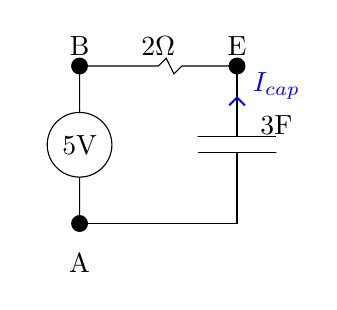
\begin{tikzpicture}
\draw (0,0)--(0,1) node[circle,draw=black, fill=white,radius=.1 mm, label=left:{}]{5V}
--(0,2)--(1,2)--(1.1,2.1)--(1.2,1.9)--(1.3,2)--(2,2);
\draw (2,2)--(2,1.1)--(1.5,1.1)--(2.5,1.1) (1.5,.9)--(2.5,.9)--(2,.9)--(2,0)--(0,0);
\draw node at (2.5,1.25) {3F};
\draw node at (1,2.25) {$2\Omega$};
\filldraw (0,0) circle[radius=1 mm];\draw node at (0,-.5) {A};
\filldraw (0,2) circle[radius=1 mm];\draw node at (0,2.25) {B};
\filldraw (2,2) circle[radius=1 mm];\draw node at (2,2.25) {E};
\draw [draw=blue,line width=.25mm] (1.9,1.5)--(2,1.6)--(2.1,1.5);
\draw node[text=blue] at (2.5,1.75) {$I_{cap}$};
\end{tikzpicture}
\caption{Voltage source connected to a capacitor with resistor}
\label{F:6CB}
\end{center}
\end{figure}

Let's determine the voltage across the capacitor as a function of time. Use nodal analysis and set node A as the reference. Node B must then be 5V, so we just need to write a nodal equation for node E.

\begin{align}
\frac{5-E}{2}+I_{cap}=0 &&\text{Currents into Node E}
\end{align}

But how to we write $I_{cap}$? We need the equation for $I_{cap}$ based on the I-V relationship for a capacitor, $I=C\frac{dV}{dt}$. The voltage difference across the capacitor, in the direction of the $I_{cap}$ is $V = (0-E)$. So, $I_{cap}=C\frac{d(0-E)}{dt}$ and our node equation then becomes:

\begin{align}
\frac{5-E}{2}-3\frac{dE}{dt}=0 &&\text{Node C} \label{E:6RC}
\end{align}

Just need to solve this equation for the voltage E(t), and we're done.

\begin{alevel}
What are the units of E? What are the units of the `5'? What are the units of the `2'?
\end{alevel}

There are lots of ways to solve this. The philosophy of this book is that the best approach is to learn several methods. The next three subsections outline three different ways to solve it. We will learn a fourth method later on \footnote{The fourth method uses Laplace Transforms. Because this technique is usually covered close to the end of the semester, this book delays its introduction. I'm not sure this is a good reason.}.

%%%%%%%%%%%%%%%%%%%%%%%%%%%%%%%%%%%%%%%%%%%%%%%%%%%%%%%%%%%%%%%%%%%%%%%%%%%%%
\subsection{Solving Strategy I: Separation of Variables}
Get all terms with the variable E to one side and those with the variable t to the other. Then integrate both sides.

\begin{align}
\frac{5-E}{2}-3\frac{dE}{dt}&=0 &\text{Node C} \notag\\
5-E&=6\frac{dE}{dt}\notag\\
dt &=6\frac{dE}{5-E}\notag\\
\int_0^{t} dt &= 6\int_{E_i}^{E} \frac{dE}{5-E} \notag\\
\frac{dt}{6}&= -(ln(5-E)-ln(5-E_i)\notag\\
-\frac{t}{6}&=ln(\frac{5-E}{5-E_i})\notag\\
(5-E_i)e^{-\frac{t}{6}}&=5-E\notag\\
E&=5-(5-E_i)e^{-\frac{t}{6}} \label{E:6RCSOL}
\end{align}

\begin{alevel}
What are the units of the '5'? What are the units of the $E_i$? What are the units of the '6'?
\end{alevel}

\begin{blevel}
After a very long time, what is the value of E?
\end{blevel}

\begin{blevel}
Assuming the initial voltage across the capacitor is zero, how much time until the voltage across the capacitor reaches 4.5 Volts?
\end{blevel}

Let's graph it.

\par
\begin{figure}[H]
\begin{center}
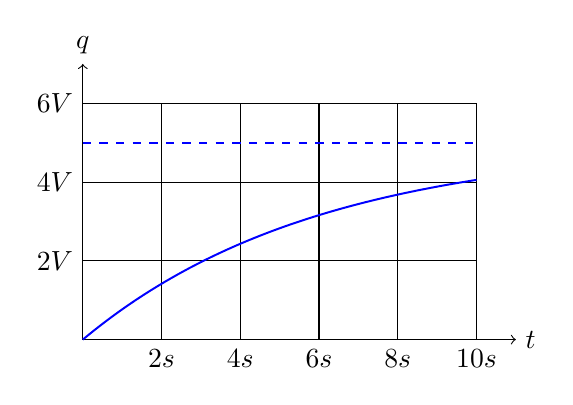
\begin{tikzpicture}
\draw[->] (0,0)--(5.5,0) node[right] {$t$};
\draw[->] (0,0)--(0,3.5) node[above] {$q$};
\draw (0,1)node[left] {$2 V$} --(5,1);
\draw (0,2)node[left] {$4 V$}--(5,2) ;
\draw (0,3)node[left] {$6 V$}--(5,3) ;
\draw (1,0)node[below] {$2 s$}--(1,3) ;
\draw (2,0)node[below] {$4 s$}--(2,3) ;
\draw (3,0)node[below] {$6 s$}--(3,3) ;
\draw (4,0)node[below] {$8 s$}--(4,3) ;
\draw (5,0)node[below] {$10 s$}--(5,3) ;
\draw [draw=blue, line width=.25 mm,smooth, samples=100,domain=0:10,scale=.5] plot(\x,{5-5*exp(-\x/6)});
\draw [draw=blue, line width=.25 mm, dashed] (0,2.5)--(5,2.5);
\end{tikzpicture}
\caption{Voltage at E over time for first 10 seconds}
\end{center}
\end{figure}

After a very long time, the voltage approaches 5V, but it never gets there (5V is a horizontal asymptote). Increased voltage across the capacitor means less voltage across the resistor. Smaller voltage across the resistor means less current. Less current means the capacitor will charge even slower.

\begin{clevel}
Fill in the following table:
\end{clevel}

\begin{table}[H]
\begin{center}
\begin{tabular}{|c|c|c|c|c|c|} \hline
time&$V_C$&$V_R$&$I_R$&extra charge delivered to C during next 0.01 s&rise in $V_C$ during next 0.01 s \\ \hline
2s&&&&& \\ \hline
20s&&&&& \\ \hline
\end{tabular}
\caption{Comparison of charging rate for a capacitor}
\end{center}
\end{table}

\begin{clevel}
Repeat the problem of solving for E(t), but for the case where the resistor is R and the size of the capacitor is C. As before, solve for the voltage across the capacitor as a function of time.
\end{clevel}

%%%%%%%%%%%%%%%%%%%%%%%%%%%%%%%%%%%%%%%%%%%%%%%%%%%%%%%%%%%%%%%%%%%%%%%%
\subsection{Solving Strategy II: Two part solution.}
Let's solve by a different method. If you're not already comfortable with this method, pay careful attention because it has many applications. We're ultimately trying to solve Equation~\eqref{E:6RC}:

\begin{align}
\frac{5-E}{2}-3\frac{dE}{dt}&=0 \notag
\end{align}

But let's start with this simpler one, so that we can focus on the important ideas at work.

\begin{align}
3x+y&=5
\end{align}

First, any solution must specify values for \textbf{both} x and y. I'll call this solution, z, and I'll write it as a column vector \footnote{Or a tuple, if you prefer. It is not a technically vector, since x and y might represent the sales of sheep and cattle. But introductory engineers can relate to vectors so I'm going with the that, imperfect as it may be.} $\vec{z}= \begin{vmatrix}x\\y\end{vmatrix}$.\\
\\
The idea is to split the solution into two parts, $\vec{z_H}$ (called the homogeneous solution) and $\vec{z_P}$ (called the particular solution).
\begin{itemize}
\item $\vec{z_H}$ will be a set of solutions including \textbf{all} combinations of x and y such that $3x+y=0$. 
\item $\vec{z_P}$ will consist of \textbf{any} one combination of x and y such that $3x+y=5$.
\end{itemize}

To be part of $\vec{z_H}$, the value of y needs to be -3x, like (x=2 and y=-6) or (x=10 and y=-30). For our example, any $\vec{z}$ in this form will work: 

\begin{align}
\vec{z_H}= \begin{vmatrix}a\\-3a\end{vmatrix}=a\begin{vmatrix}1\\-3\end{vmatrix}
\end{align} 

Note, the solution (x=3,y=-9) would be a member of $\vec{z_H}$ but not $z$ ($\vec{z_H}$ is a solution to 3x+y=0, not 3x+y=5).\par

As for $\vec{z_P}$, well, we just need to find one, not all, of the possibilities. The easiest might be: $\vec{z_P}= \begin{vmatrix}0\\5\end{vmatrix}$. Putting it all together means the solution is:\\

\begin{align*}
\vec{z}=\vec{z_H}+\vec{z_P}\\
\vec{z}= a\begin{vmatrix}1\\-3\end{vmatrix}+\begin{vmatrix}0\\5\end{vmatrix}.
\end{align*} 

\begin{blevel}
Identify any three solutions for $\vec{z}$.
\end{blevel}

To help see why this works and also importantly, when it works, let's repackage our equation into function notation like so:

\begin{align*}
3x+y&=5\\
f(x,y)&=5	&&\text{In function notation}\\
f(\vec{z})&=5	&&\text{Write x and y as $\vec{z}$}\\
f(\vec{z_H}+\vec{z_P})&=5	&&\text{Split $\vec{z}$ into parts}\\
f(\vec{z_H})+f(\vec{z_P})&=5 &&\text{Key Step}\\
0+5&=5	&&\text{The two parts do their jobs}
\end{align*}

Examine the key step. This does NOT always work - it only works for linear functions.

\begin{alevel}
What would be f(2,5)?
\end{alevel}

\begin{alevel}
What would be $f(\vec{Z_H}+\vec{Z_H})$? What would be $f(\vec{Z_P}+\vec{Z_P})$?
\end{alevel}

\begin{clevel}
Solve $5x - 2y = 20$ using the same method. Find $z_H$ and $z_P$. 
\end{clevel}

\begin{dlevel}
Solve $5x - 2y = 20$ using the same method. If two engineers correctly find $z_H$ and $z_P$, will they get the same $z_H$'s? Will they get the same $z_P$'s?
\end{dlevel}

We could write this in matrix notation as follows:

\begin{align*}
3x+y&=5\\
\begin{vmatrix}3&1\end{vmatrix} \begin{vmatrix}x \\ y\end{vmatrix} &=5\\
A\vec{z}&=5\\
A(\vec{z_H}+\vec{z_P})&=5\\
A\vec{z_H}+A\vec{z_P}&=5\\
0+5&=5
\end{align*}

\begin{alevel}
What is the shape of the matrix labeled A?
\end{alevel}

\begin{clevel}
What would be $A(\vec{z_H}+\vec{z_H})$? How about $A(\vec{z_P}+\vec{z_P})$?
\end{clevel}

Now, we're ready to go back and attack the equation at hand.

%%%%%%%%%%%%%%%%%%%%%%%%%%%%%%%%%%%%%%%%%%%%%%%%%%%%%%%%%%%%%%%%%%%%%
\subsection{Solving Strategy II: Implementation}
We begin by rewriting the equation into a suitable form:
\begin{align*}
\frac{5-E}{2}-3\frac{dE}{dt}=0 &&\text{Node C}\\
E+6\frac{dE}{dt}=5 &&\text{After rearrangement}\\
E+6\frac{dE}{dt}=0 &&\text{Homogeneous Equation (needs ALL solutions)}\\
E+6\frac{dE}{dt}=5 &&\text{We need just any solution to this}
\end{align*}

Our solution will be the sum of two parts, $E=E_H+E_P$. We now need to determine the two pieces. 


\begin{itemize}
\item \underline{Finding $E_H$:}\\
We need to solve:
\begin{align*}
E+6\frac{dE}{dt}=0 &&\text{Homogeneous Equation}\\
\end{align*}

We make an assumption about the form of $E_H$. We assume a form of $E_H=Ae^{mt}$. This might seem rather limiting, but we've got two parameters to play with, A and m. The upside is that this function is easy to work with. Substituting back into the homogeneous equation gives:\\

\begin{align*}
E+6\frac{dE}{dt}=0 \\
Ae^{mt} + 6mAe^{mt} =0\\
1+6m=0\\
m = -\frac{1}{6}\\
E_H=Ae^{-\frac{t}{6}}
\end{align*}

So $E_H = Ae^{-\frac{1}{6}t}$.  We'll find the value of A later.
 
\item \underline{Finding $E_P$:}\\
There can be a bit of skill to finding a particular solution. For many situations, the following rule of thumb works: Guess a function that is of the same form as f(t) on the right side of the equation. In our case, f(t) is a constant, so we'll guess $E_P=k$. Plug in to Equation~\eqref{E:6RC} and solve for k.

\begin{align*}
E+6\frac{dE}{dt}=5=f(t) \\
k + 6*0 =5\\
k=5\\
E_P=5 &&\text{because $E_P=k$}
\end{align*}

\end{itemize}

Because $E=E_H+E_P$, then $E=Ae^{-\frac{1}{6}t}+5$. The last thing to do is use initial conditions to find any unknown constants.\footnote{Initial conditions must be plugged into the total solution for E, not into just $E_P$ or $E_H$.} Our capacitor started off at $E=E_i$ Volts, or $E(t=0)=E_i$. Plug this in and solve for A.

\begin{align*}
E=Ae^{-\frac{1}{6}t}+5 \\
0=Ae^{0}+5\\
A=-5
\end{align*}

Finally, in all its glory: $E = -5e^{-\frac{1}{6}t}+5$. This, of course, matches what we got from the first method.

\begin{blevel}
As time goes to infinity, what happens to $E_H$? What happens to $E_P$?
\end{blevel}

\begin{clevel}
Solve this equation using this method: $3I + 2\frac{dI}{dt}=10$. Separately list $I_H$ and $I_P$.
\end{clevel}



%%%%%%%%%%%%%%%%%%%%%%%%%%%%%%%%%%%%%%%%%%%%%%%%%%%%%%%%%%%%%%%%%%%%%%%%
\subsection{Solving Strategy III: Exact Differentials}

Some equations that engineers and scientists bump into are in a form called exact differential equations. Of the ones that aren't, many can be made to be exact by multiplying both sides of the equation by something called an integrating factor. This section demonstrates this method to solve the same equation that we have already twice solved.\\

An exact differential equation takes the form:$M(x,y)dx + N(x,y)dy = 0$ where $\frac{dM}{dy}=\frac{dN}{dx}$. If it is exact, it may be easy to solve and the resulting function would have some nice properties. \footnote{Like being path independent, and therefore lead to a potential function.}

\begin{blevel}
Which of the following differential equations are exact?
\begin{enumerate}
\item $3dx + 3dy = 0$
\item $3dx + 2dy = 0$
\item $3xdx + 3ydy = 0$
\item $3ydx + 3xdy = 0$
\item $3x^2dx + 3y^2dy = 0$
\item $3y^2dx + 3x^2dy = 0$
\item $(y-5)dx + 3dy = 0$
\item $k_1dT+\frac{k_2}{V}dV=0$
\end{enumerate}
\end{blevel}

Let's test the equation that we've been working on, Equation~\eqref{E:6RC}, for exactness. Notice that our variables are E and t, not x and y. We'll need to rearrange it a little to make it match $M(x,y)dx + N(x,y)dy = 0$.

\begin{align}
\frac{5-E}{2}-3\frac{dE}{dt}&=0 &&\text{Node C}\notag\\
E+6\frac{dE}{dt}&=5 \notag\\
Edt+6dE&=5dt \notag\\
(E-5)dt+6dE&=0 &&M(E,t)dt+N(E,t)dE=0 \label{E:6RCEX}
\end{align}

\begin{blevel}
Show that Equation~\eqref{E:6RCEX} is not exact.
\end{blevel}

If a linear first order differential equation is not exact, we can make it exact by multiplying the equation by a function (we'll call it $\mu(t)$). This function is called an integrating factor.

\begin{align*}
(E-5)dt+6dE&=0\\
\mu(t)(E-5)dt+\mu(t)6dE&=0
\end{align*}

We wish to pick $\mu(t)$ so that the equation becomes exact.

\begin{align*}
\frac{dM}{dE}=\frac{dN}{dt}\\
\frac{d(\mu(t)(E-5))}{dE}=\frac{d(\mu(t)6)}{dt}\\
\mu(t)=6\frac{d\mu(t)}{dt}\\
\frac{1}{6}dt=\frac{d\mu(t)}{\mu(t)}\\
\int \frac{1}{6}dt=\int \frac{d\mu(t)}{\mu(t)}\\
\frac{1}{6}t=\ln(\mu(t))\\
\mu(t)=e^{\frac{1}{6}t}
\end{align*}

Now we have our integrating factor, multiply it through and get:

Executing this plan:
\begin{align}
\mu(t)(E-5)dt+\mu(t)6dE&=0 \notag\\
e^{\frac{t}{6}}(E-5)dt+e^{\frac{t}{6}}6dE&=0 \label{E:6NT3}
\end{align}

\begin{blevel}
Show that Equation~\eqref{E:6NT3} is exact.
\end{blevel}

Next, determine what function would lead to this differential. We know that when we take a derivative w.r.t. x, we get M. When we take a derivative w.r.t. y, we get N. Therefore we can uncover the fucntion by integrating M w.r.t. x and N w.r.t. y. Then keep all the terms, but not duplicates. A more thorough discussion can be found in a differential equations text.\footnote{I'm not really trying to cover it here, just reenforcing what the reader might have seen in a differential equation class. Second, exact differentials will surface again in thermodynamics and other places.}\\

Executing this plan:
\begin{align*}
e^{\frac{t}{6}}(E-5)dt+e^{\frac{t}{6}}6dE&=0\\
\int e^{\frac{t}{6}}(E-5) dt &= 6e^{\frac{t}{6}}(E-5)\\
\int e^{\frac{t}{6}}6 dE &= 6e^{\frac{t}{6}}E\\
k &= 6e^{\frac{t}{6}}(E-5) \tag{Keep all terms, not duplicates}\\
k_2e^{-\frac{t}{6}}&=E-5\tag{Solve for E}\\
E &= 5-k_2e^{-\frac{t}{6}}
\end{align*}

Finally, use the initial condition ($E(t=0)=0$) to find $k_2$.

\begin{align*}
E &= 5-k_2e^{-\frac{1}{6}t}\\
0 &= 5-k_2\\
k_2&=5\\
E &= 5-5e^{-\frac{1}{6}t}
\end{align*}

\begin{clevel}
Repeat this process for solving the following equation: $3I + 2\frac{dI}{dt}=10$. What did the integrating factor turn out to be?
\end{clevel}

%%%%%%%%%%%%%%%%%%%%%%%%%%%%%%%%%%%%%%%%%%%%%%%%%%%%%%%%%%%
\section{A timer circuit}
In this section, we'll design a circuit with a purpose. Goal: When a switch is closed, we wish a light to turn on for 10 seconds and then abruptly turn off.\\

How do we design such a circuit? First, consider some concepts we might draw on. 

\begin{itemize}
\item We want something to abruptly trigger a change in voltage level. This seems like an op-amp.
\item We need something that will cause a voltage to change with time, so that after 10s we can trigger the op-amp. This could be an RC circuit.
\end{itemize}

Here's our design so far. We'll connect the op-amp power supplies to +5V and -5V (not shown on diagram).

\begin{figure}[H]
\begin{center}
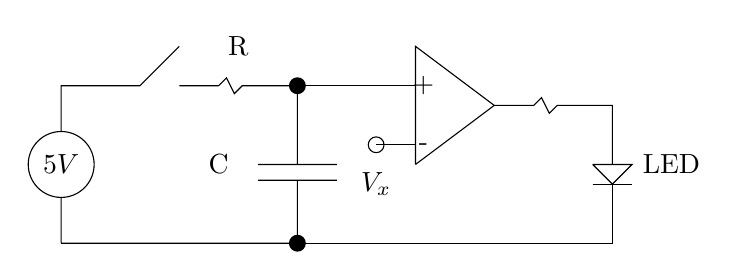
\begin{tikzpicture}
\draw (0,0)--(0,1) node[circle, draw=black,fill=white]{$5V$}--(0,2)
--(1,2)--(1.5,2.5) (1.5,2)--(2,2)--(2.1,2.1)--(2.2,1.9)--(2.3,2)--(3,2)
--(3,1)--(2.5,1)--(3.5,1) (3.5,.8)--(2.5,.8)--(3,.8)--(3,0)--(0,0);
\filldraw (3,2) circle[radius=1 mm];
\filldraw (3,0) circle[radius=1 mm];
\draw (4,1.25) circle[radius=1 mm];
\draw node at (2.25,2.5) {R};
\draw node at (2,1) {C};
\draw node at (7.75,1) {LED};
\draw node at (4.6,2) {+};
\draw node at (4.6,1.25) {-};
\draw node at (4,.75) {$V_x$};
\draw (3,2)--(4.5,2);
\draw (4,1.25)--(4.5,1.25);
\draw (4.5,1)--(4.5,2.5)--(5.5,1.75)--(4.5,1);
\draw (5.5,1.75)--(6,1.75)--(6.1,1.85)--(6.2,1.65)--(6.3,1.75)--(7,1.75)
--(7,1)--(6.75,1)--(7.25,1)--(7,.75)--(6.75,1);
\draw (6.75,.75)--(7.25,.75);
\draw (7,.75)--(7,0)--(0,0);
\end{tikzpicture}
\caption{Schematic for timer circuit. First attempt.}
\end{center}
\end{figure}

When the switch is closed, the voltage across the capacitor will start to rise. While it is less than $V_x$, the op-amp will try to produce $-\infty V$ (but it will only actually reach the negative power supply voltage for the op-amp, -5V). In this case, the diode would be biased in the reverse direction. No current will flow and the light would be off. \\

When the voltage across the capacitor exceeds $V_x$, the output of the op-amp will switch to +5V volts and the LED will turn on.\footnote{A resistor is connected in series with the LED to limit the current (~50 Ohms).} \\

We still need to make the following design tweaks:
\begin{enumerate}
\item The design is backwards. The light is supposed to be on for 10s, then off. The current design is off, then on. We fix this by reversing the op-amp inputs.
\item Timing isn't exactly 10 seconds. We could pick $R=100,000\Omega$ and $C=10\mu F$ and then calculate the voltage across the capacitor after 10 s. Then, we'll set $V_x$ to that value.
\end{enumerate}

When analyzing this RC circuit we recall that no significant current goes into the op-amp input terminals. This lets us ignore the op-amp for the RC circuit analysis. The analysis proceeds in a similar way as covered earlier in this chapter. The equation for $V_C(t)$ would be:\\

\begin{align*}
V_C &= 5 - 5e^{-t}\\
V_C(t=10s)&=4.999773 V
\end{align*}

We conclude that we should set Vx to 4.999773 V. Well, this might work with some \textbf{very precise equipment}, but setting $V_x$ to 4.999773V instead of 4.9721V would be a real challenge. Let's make the circuit more workable by slowing down the charging rate of the capacitor. We can do this by making the resistor 100x bigger.

\begin{clevel}
Calculate the new equation for $V_C(t)$.
\end{clevel}

\begin{clevel}
Determine the new value to set for $V_x$. Redraw the whole timer circuit, with all the tweaks.
\end{clevel}
%%%%%%%%%%%%%%%%%%%%%%%%%%%%%%%%%%%%%%%%%%%%%%%%%%%%%%%%%%%%%%%%%%%%%
\section{Mechanical Analog to RC Circuit}
Earlier, we said that a capacitor acts like a spring. Is there a mechanical system that behaves like an RC circuit? Yes. Consider a massless object connected to a spring. If you pull the object away to the right a little bit, it will tend to spring back to its original position. The effect of air drag \footnote{Or fluid drag, if the object were immersed in a liquid.} resembles the resistance in the RC circuit. We'll use $F=-bv$ as our air drag model; such a model makes the drag force behave mathematically just like a resistor.\par

\begin{figure}[H]
\begin{center}
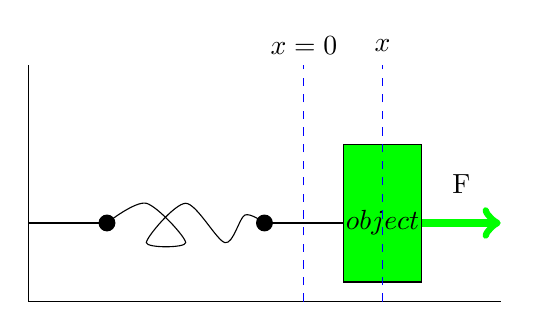
\begin{tikzpicture}
\draw (0,0)--(0,3) (0,0)--(6,0);
\draw [draw=black, fill=green] (4,.25) rectangle (5,2);
\filldraw (3,1) circle[radius=1 mm];
\draw plot [smooth] coordinates {(1,1) (1.5,1.25) (2,.75) (1.5,.75) (2,1.25) (2.5,.75) (2.75,1.1) (3,1)};
\filldraw (1,1) circle[radius=1 mm];
\draw node at (4.5,1) {$object$};
\draw (3,1)--(4,1) (0,1)--(1,1);
\draw node at (4.5,3.25) {$x$};
\draw node at (3.5,3.25) {$x=0$};
\draw [dashed, draw=blue] (4.5,0)--(4.5,3) (3.5,0)--(3.5,3);
\draw [draw=green, line width=1 mm] [->] (5,1)--(6,1);
\draw [draw=green] node at (5.5,1.5) {F};
\end{tikzpicture}
\caption{Mechanical Analog to RC circuit. Massless object on spring with frictional drag.}
\label{F:6RCM}
\end{center}
\end{figure}

In the RC circuit that we studied in Figure~\ref{F:6CB}, the capacitor started uncharged. This would be equivalent to the object starting at unstretched position. Then, we suddenly connected a voltage across the RC circuit. For us, this would be like suddenly applying a constant force to the mass, shown in green on Figure~\ref{F:6RCM}.\par

Set the contant force to 5N, the spring constant to 1 N/m and the drag coefficient to b=6 N*s/m. Writing out F=ma:

\begin{align*}
F_T=ma=m\frac{dv}{dt}=m\frac{d(\frac{dx}{dt})}{dt}=m\frac{d^2x}{dt^2}=0&&\text{Because mass=0}\\
F-kx-bv=0\\
5-x-6\frac{dx}{dt}=0\\
x+6\frac{dx}{dt}=5
\end{align*}

Compare this with equation~\eqref{E:6RC} and you can see the likeness \footnote{The numbers, of course, have different units and the variable is x instead of the voltage at E.}

The solution for x(t) must then be equation~\eqref{E:6RCSOL}.

\begin{align}
x(t)=5-5e^{-\frac{t}{6}}
\end{align}

\begin{alevel}
What are the units of the the first '5'?
\end{alevel}

\begin{blevel}
Where is the mass after 10 seconds?
\end{blevel}

The following table shows some analogous quantities/relationships between electrical and mechanical system:

\begin{table}[H]
\begin{center}
\begin{tabular}{|c|c|} \hline
electrical& mechanical \\ \hline
q&x \\ \hline
$i=\frac{dq}{dt}$& $v=\frac{dx}{dt}$ \\ \hline
V&F\\ \hline
$V=\frac{1}{C}q$&F=-kx\\ \hline
$\frac{1}{C}$&k\\ \hline
V=RI&F=-bv\\ \hline
R&b\\ \hline
\end{tabular}
\caption{Mechanical and Electrical Analogous Quantities and Relationships}
\end{center}
\end{table}

Consider two analogous sytems:
\begin{enumerate}
\item An electrical circuit: A 10V source connected in series with a 3 $\Omega$ resistor and a 7 F capacitor.
\item A mechanical system: A massless plate connected to a spring (k = 1/7 N/m) and being pulled to the right by a 10 N force. The is a drag force of $F_D=-3v$.
\end{enumerate}
These two systems are governed by the same equation.
\begin{enumerate}
\item The electrical circuit:
\begin{align*}
\frac{10-V_C}{3}+7\frac{d}{dt}(0-V_C)=0&&\text{From Nodal Analysis}\\ 
\rightarrow 10=21\frac{d}{dt}V_C+V_C \\
\rightarrow 10=3\frac{d}{dt}Q_C+\frac{Q_C}{7}&&\text{Using $V_C = \frac{Q_C}{C}$}.
\end{align*}
\item A mechanical system: 
\begin{align*}
F_T=ma \rightarrow 10-3v-\frac{1}{7}x=0*a \\
\rightarrow 10=3\frac{d}{dt}x+\frac{1}{7}x
\end{align*}
\end{enumerate}

If they both start with a similar initial state ($V_C=0$ and $x_i=0$), then their solutions will also be the same: $Q_C=\frac{10}{7}-\frac{10}{7}e^{-\frac{t}{21}}$ Coulombs or $x=\frac{10}{7}-\frac{10}{7}e^{-\frac{t}{21}}$ meters.

\begin{clevel}
Determine both a mechanical problem and an RC circuit that result in this equation:$x(t),q(t)=2-2e^{-\frac{t}{3}}$
\end{clevel}

\begin{dlevel}
Determine both a mechanical problem and an RC circuit that result in this equation:$x(t)=2-4e^{-\frac{t}{3}}$. Hint: Think about the initial conditions.
\end{dlevel}


%%%%%%%%%%%%%%%%%%%%%%%%%%%%%%%%%%%%%%%%%%%%%%%%%%%%%%%%%%%%%%%%%%%%%
\section{Inductors}
An inductor behaves as the dual for the capacitor, its I-V relationship is similar, but with the roles of current and voltage reversed ($V=L\frac{dI}{dt}$). When the current through an inductor tries to change, a voltage is developed across the inductor to try to keep the current going the way it had been going (a magnetic effect). The magnitude of this voltage is proportional to how fast the current changes.\\
\\
A circuit with inductance behaves like a mechanical system with mass. Mass requires force to change its velocity. Inductors require voltage to change thier current. The following set of equations tries to highlight some similarities between inductance and mass.

\begin{align*}
F = m\frac{dv}{dt}&&V=L\frac{dI}{dt}\\
F = m\frac{d^2 x}{dt^2}&&V=L\frac{d^2 q}{dt^2}
\end{align*}

\begin{alevel}
What are the units of magnetic field?
\end{alevel}

\begin{blevel}
What is the approximate strength of the Earth's magnetic field?
\end{blevel}

\begin{clevel}
A wire has 10A of current flowing through it. What is the magnetic field strength 1 cm away from the wire?
\end{clevel}

\begin{alevel}
A 5H inductor has a steady current of 10Amps passing through it. What is the voltage drop across this inductor?
\end{alevel}

\begin{blevel}
A 5H inductor has a steady current of 10Amps passing through it. What must be the voltage across the inductor in order to increase the current to 15 Amps in 5 seconds? 
\end{blevel}

Let's analyze the circuit shown in Figure~\ref{F:6RL0} to determine the current as a function of time. Let's leave R and L as variables.

\begin{figure}[H]
\begin{center}
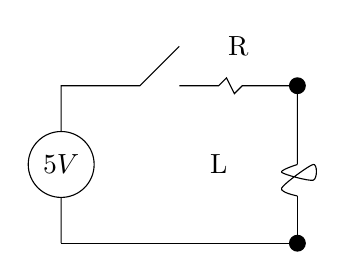
\begin{tikzpicture}
\draw (0,0)--(0,1) node[circle, draw=black,fill=white]{$5V$}--(0,2)
--(1,2)--(1.5,2.5) (1.5,2)--(2,2)--(2.1,2.1)--(2.2,1.9)--(2.3,2)--(3,2)
--(3,1);
\draw plot [smooth] coordinates {(3,1) (2.8,.9) (3.2,.8) (3.2,1) (2.8,.7) (3,.6)};
\draw (3,.6)--(3,0)--(0,0);
\filldraw (3,2) circle[radius=1 mm];
\filldraw (3,0) circle[radius=1 mm];
\draw node at (2.25,2.5) {R};
\draw node at (2,1) {L};
\end{tikzpicture}
\caption{RL circuit}
\label{F:6RL0}
\end{center}
\end{figure}

We'll use loop analysis.

\begin{align}
5-IR - L\frac{dI}{dt}=0
\end{align}

Of the three methods for solving (best to use all three), I'll use method II and begin by determining the two parts of the solution:$I_C$ and $I_P$.

\begin{align*}
5-IR - L\frac{dI}{dt}=0\\
L\frac{dI}{dt}+IR = 5\\
L\frac{dI}{dt}+IR = 0 &&\text{Homogeneous Equation, solve for $I_C$}
\end{align*}

To find $I_H$ let $I_H=Ae^{mt}$. Plug in and solve for m ($m=-\frac{R}{L}$). So, $I_C=Ae^{-\frac{R}{L}t}$.\\

To find $I_P$ let $I=k$ and plug in to entire equation and solve for k ($k=\frac{5}{R}$). Putting these together gives: $I = \frac{5}{R}+Ae^{-\frac{R}{L}t}$. Finally, we use an initial condition to solve for A $I(0)=0 \rightarrow A=-\frac{5}{R}$.

\begin{align*}
I = \frac{5}{R}-\frac{5}{R}e^{-\frac{R}{L}t}
\end{align*}

\begin{blevel}
What happens to $I_C$ as $t \rightarrow \infty$? What happens to $I_P$ as $t \rightarrow \infty$? What happens to $I$ as $t \rightarrow \infty$?
\end{blevel}

\begin{blevel}
As $t \rightarrow \infty$, what basic component does the inductor seem to act like?
\end{blevel}

\begin{blevel}
According to the equation, what must be the units of $\frac{L}{R}$?
\end{blevel}

%%%%%%%%%%%%%%%%%%%%%%%%%%%%%%%%%%%%%%%%%%%%%%%%%%%%%%%%%
\section{Finding initial conditions}
In this section, we need to justify two observations:

\begin{enumerate}
\item The voltage across a capacitor can not change instantly (but it can change very fast).
\item The current through an inductor can not change instantly (but it can change very fast).
\end{enumerate}

These statement are based on the fact that both $\Delta V_C$ and $\Delta I_L$ are determined by integrals over time (see Table~\ref{T:6RLC}). If no time has transpired, the integrals over time must evaluate to zero. This would be true to any integral with a non-infinite integrand.\\

\begin{align}
\int_{t=t_1}^{t=t_2}(something)dt=0&&\text{If $t_1$=$t_2$}
\end{align}

\begin{blevel}
What is: $\int_{4}^{5}x^2dx$? What is: $\int_{5}^{5}x^2dx$?
\end{blevel}

\begin{blevel}
A car, initially driving at 20 m/s accelerates at 10 $\frac{m}{s^2}$ for zero seconds. What is the final speed of the car?
\end{blevel}

Let's look at the circuit in Figure~\ref{F:6RL}, but this time start with the switch closed and then suddenly open it at t=0s.

\begin{figure}[H]
\begin{center}
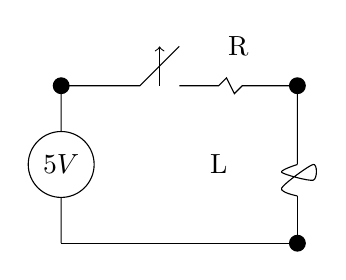
\begin{tikzpicture}
\draw (0,0)--(0,1) node[circle, draw=black,fill=white]{$5V$}--(0,2)
--(1,2)--(1.5,2.5) (1.5,2)--(2,2)--(2.1,2.1)--(2.2,1.9)--(2.3,2)--(3,2)
--(3,1);
\draw plot [smooth] coordinates {(3,1) (2.8,.9) (3.2,.8) (3.2,1) (2.8,.7) (3,.6)};
\draw (3,.6)--(3,0)--(0,0);
\draw [->] (1.25,2)--(1.25,2.5);
\filldraw (0,2) circle[radius=1 mm];
\filldraw (3,2) circle[radius=1 mm];
\filldraw (3,0) circle[radius=1 mm];
\draw node at (2.25,2.5) {R};
\draw node at (2,1) {L};
\end{tikzpicture}
\caption{RL Circuit}
\label{F:6RL}
\end{center}
\end{figure}

It might be useful to make a table of all currents and voltages in the circuit just before ($t=0_{-}$) and just after the switch opens ($t=0_{+}$).

\begin{table}[H]
\begin{center}
\begin{tabular}{|c|c|c|c|c|} \hline
object	&$I(t=0_{-})$	&$V(t=0_{-})$	&$I(t=0_{+})$	&$V(t=0_{+})$ \\ \hline
5V source&&&& \\ \hline
switch&&&& \\ \hline
R&&&& \\ \hline
L&&&& \\ \hline
\end{tabular}
\caption{Initial condition table. Switch starts closed and then opens.}
\end{center}
\end{table}

One possible sequence of analysis to fill in the table would be as follows.
\begin{enumerate}
\item Before the switch is opened the voltage across the 5V source is, of course, 5V. 
\item Before the swtich is opened, the closed switch is a perfect wire, so the voltage across it is zero. 
\item The voltage across the inductor is $V_L=L\frac{dI}{dt}$. If the circuit has been sitting there for a while and nothing is changing \footnote{There is an assumption here, some unattended circuits could still have changing currents. We'll have to fall back on this RL circuit and the equation we derived for it as $t \rightarrow \infty$.} then the derivative is zero and the voltage across the inductor is zero. 
\item By KVL, the voltage across the resistor must then be 5V.
\item Using Ohm's law, the current through the resistor is $\frac{5}{R}$ Amps.
\item Then the current through the 5V supply, the switch and the inductor must all be $\frac{5}{R}$.\footnote{Note that even though the voltage across the inductor is zero, the current through it is not.}
\end{enumerate}

Now what about just after the switch opens (time $t=0_{+}$)?\\
\begin{enumerate}
\item Identify which quantities can NOT change instantly. The current through an inductor can not change instantly, therefore it will remain $\frac{5}{R}$ Amps.
\item The current through the 5V source and resistor must also be $\frac{5}{R}$ Amps.
\item Here is the big reveal - the current through the open switch must also be $\frac{5}{R} Amps$! At least for an instant.
\item The voltage across the 5V source is still 5V.
\item After using Ohm's law, we see that the voltage across the resistor is still 5V.
\item The voltage across the switch is now the current times the resistance of the air gap (maybe 1 MILLION Ohms). So $V_{switch}=\frac{5}{R}*1000000$ Volts. Depending on the size of the inductor, this can be dangerous. Treat this situation with respect. The voltage is large enough that you might see a spark.
\item Use KVL to determine the voltage across the inductor at time ($t=0_+$):
\begin{align*}
5-V_{switch}-IR-V_L&=0\\
5-\frac{5000000}{R}-5-V_L&=0\\
V_L(t=0_+)&=\frac{5000000}{R}
\end{align*}
\end{enumerate}

Once the initial conditions are determined, the equation for $V_L(t)$ can be found.

\begin{blevel}
If $R=10\Omega$, find $V_L(t=0_+)$. Determine $\frac{dI}{dt}$ at this instant.
\end{blevel}

\begin{clevel}
Show that if $R=10\Omega$ that $V_L(t)=500000e^{-\frac{1,000,010}{L}t}$.
\end{clevel}

\begin{clevel}
Assuming $R=10\Omega$ and L=2H, determine the time it takes for the voltage across the inductor to be less than 1V.
\end{clevel}

\begin{clevel}
Fill in initial condition table, Table~\ref{T:6ICP}. The situation is the same as before, except now the switch starts off open and then closes at time t=0 seconds.
\end{clevel}

\begin{table}[H]
\begin{center}
\begin{tabular}{|c|c|c|c|c|} \hline
object	&$I(t=0_{-})$	&$V(t=0_{-})$	&$I(t=0_{+})$	&$V(t=0_{+})$ \\ \hline
5V source&&&& \\ \hline
switch&&&& \\ \hline
R&&&& \\ \hline
L&&&& \\ \hline
\end{tabular}
\caption{Initial condition table. Switch is initially open, then closes at t=0s.}
\label{T:6ICP}
\end{center}
\end{table}

%%%%%%%%%%%%%%%%%%%%%%%%%%%%%%%%%%%%%%%%%%%%%%%%%%%%%%%%
\section{u(t) notation}
The circuits we studied in this chapter involved switches that opened or closed at certain moments in time. In this section we'll introduce a function that captures the functionality of the switch mathematically. This function is used extensively in signal processing and other areas, and you should try to make friends with it.\par

Consider the two circuits shown in Figure~\ref{F:6SW1}. The left diagram shows a series RL circuit that switches between ground and a 5V source. The right circuit shows a series RL circuit that switches betweeen an open circuit (disconnected) and 5V. These circuits can behave differently. \footnote{The one on the left could have some current before the switch connects it to 5V, whereas the one on the right can not.}

\begin{figure}[H]
\begin{center}
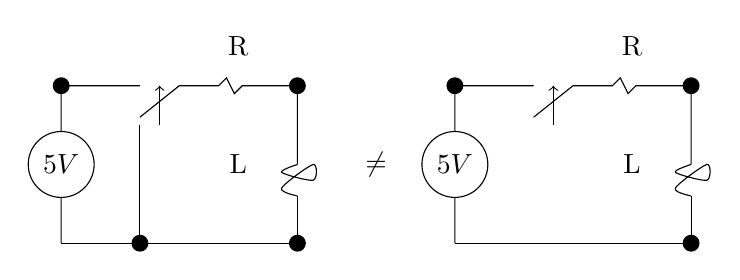
\begin{tikzpicture}
\draw (0,0)--(0,1) node[circle, draw=black,fill=white]{$5V$}--(0,2)
--(1,2)(1,1.6)--(1.5,2)--(2,2)--(2.1,2.1)--(2.2,1.9)--(2.3,2)--(3,2)
--(3,1);
\draw plot [smooth] coordinates {(3,1) (2.8,.9) (3.2,.8) (3.2,1) (2.8,.7) (3,.6)};
\draw (3,.6)--(3,0)--(0,0);
\draw [->] (1.25,1.5)--(1.25,2);
\draw (1,1.5)--(1,0);
\filldraw (1,0) circle[radius=1 mm];
\filldraw (0,2) circle[radius=1 mm];
\filldraw (3,2) circle[radius=1 mm];
\filldraw (3,0) circle[radius=1 mm];
\draw node at (2.25,2.5) {R};
\draw node at (2.25,1) {L};
\draw node at (4,1) {$\neq$};
\draw (5,0)--(5,1) node[circle, draw=black,fill=white]{$5V$}--(5,2)
--(6,2)(6,1.6)--(6.5,2)--(7,2)--(7.1,2.1)--(7.2,1.9)--(7.3,2)--(8,2)
--(8,1);
\draw plot [smooth] coordinates {(8,1) (7.8,.9) (8.2,.8) (8.2,1) (7.8,.7) (8,.6)};
\draw (8,.6)--(8,0)--(5,0);
\draw [->] (6.25,1.5)--(6.25,2);
\filldraw (5,2) circle[radius=1 mm];
\filldraw (8,2) circle[radius=1 mm];
\filldraw (8,0) circle[radius=1 mm];
\draw node at (7.25,2.5) {R};
\draw node at (7.25,1) {L};
\end{tikzpicture}
\caption{RL Circuit with two similar but different types of switches.}
\label{F:6SW1}
\end{center}
\end{figure}

The circuit on the left can be replaced with the following diagram:

\begin{figure}[H]
\begin{center}
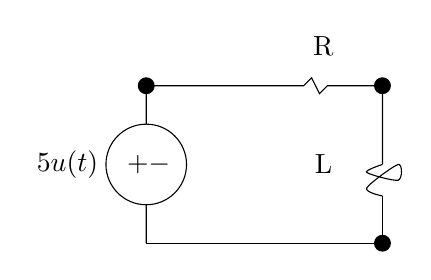
\begin{tikzpicture}
\draw node at (-1,1) {$5u(t)$};
\draw (0,0)--(0,1) node[circle, draw=black,fill=white]{$\begin{matrix}+\\-\end{matrix}$}--(0,2)--(2,2)--(2.1,2.1)--(2.2,1.9)--(2.3,2)--(3,2)--(3,1);
\draw plot [smooth] coordinates {(3,1) (2.8,.9) (3.2,.8) (3.2,1) (2.8,.7) (3,.6)};
\draw (3,.6)--(3,0)--(0,0);
\filldraw (0,2) circle[radius=1 mm];
\filldraw (3,2) circle[radius=1 mm];
\filldraw (3,0) circle[radius=1 mm];
\draw node at (2.25,2.5) {R};
\draw node at (2.25,1) {L};
\end{tikzpicture}
\caption{Switch functionality captured with u(t) function.}
\label{F:6SW1}
\end{center}
\end{figure}

The u(t) function (unit step function) is often defined as follows:

\begin{align}
u(t)=\begin{cases}
0,&\text{$x<0$}\\
1,&\text{$x>0$}\\
\frac{1}{2},&\text{$x=0$}
\end{cases}
\end{align}

\begin{alevel}
What are u(3), u(-1), u(5), u($\pi$)?
\end{alevel}

In our problem, $5u(t)$, would mean 5V for any time after 0 and 0V for any time prior. Its graph would look like Figure~\ref{F:6UT} \footnote{You might complain about how I drew the graph at t=0. The definition says it is discontinous there, shouldn't we draw the open circles and then put a dot at (0,2.5V)? We could, and maybe we should, but any oscilloscope trace will not look like that. It will look closer to this drawing and be continuous.}:

\begin{figure}[H]
\begin{center}
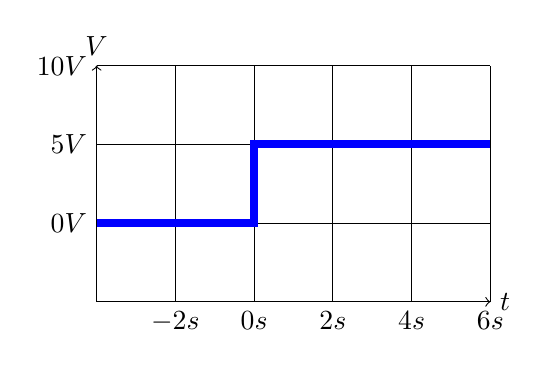
\begin{tikzpicture}
\draw[->] (0,0)--(5,0) node[right] {$t$};
\draw[->] (0,0)--(0,3) node[above] {$V$};
\draw (0,1)node[left] {$0 V$} --(5,1);
\draw (0,2)node[left] {$5 V$}--(5,2) ;
\draw (0,3)node[left] {$10 V$}--(5,3) ;
\draw (1,0)node[below] {$-2 s$}--(1,3) ;
\draw (2,0)node[below] {$0 s$}--(2,3) ;
\draw (3,0)node[below] {$2 s$}--(3,3) ;
\draw (4,0)node[below] {$4 s$}--(4,3) ;
\draw (5,0)node[below] {$6 s$}--(5,3) ;
\draw [draw=blue, line width=1 mm] (0,1)--(2,1)--(2,2)--(5,2);
\end{tikzpicture}
\caption{Graph of 5*u(t)}
\label{F:6UT}
\end{center}
\end{figure}

\begin{blevel}
Draw graphs of u(t-2), u(-t) and 3u(t+1) on the same graphic. Hint: Review your algebra skills to related to the shifting of functions.
\end{blevel}

\begin{clevel}
Make a sketch of sin(t)u(t). Separately, graph (u(t)-u(t-1)).
\end{clevel}

\begin{dlevel}
Sketch the integral of u(t). Sketch the derivative of u(t).
\end{dlevel}


